% %COPY OD ARANI's FINAL DOC BEFORE JHELUM"S EDIT

% \section{Effects on Family}

% \begin{figure}[h!]
% 	\centering
% 	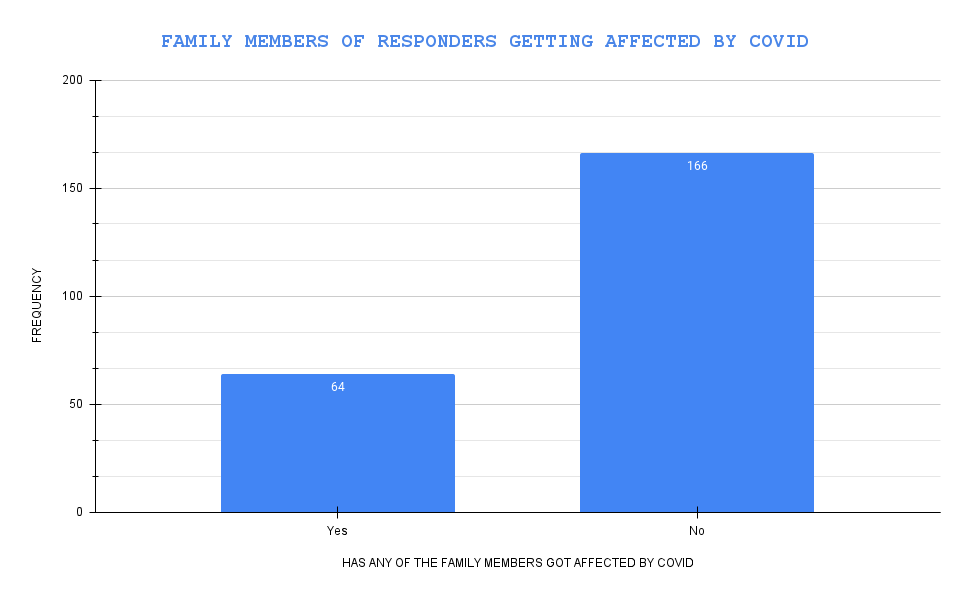
\includegraphics[width=0.45\linewidth]{IMAGES/Image 26.png}
% 	\caption{Effected by COVID in Family}
% 	\label{G26}
% \end{figure}

% \

% Figure \ref{G26} represents that 64 participants have reported having family members have been affected by COVID-19, while the remaining 166 participants indicated that none of their family members had been impacted by the virus.

% \ 

% \begin{figure}[h!]
% 	\centering
% 	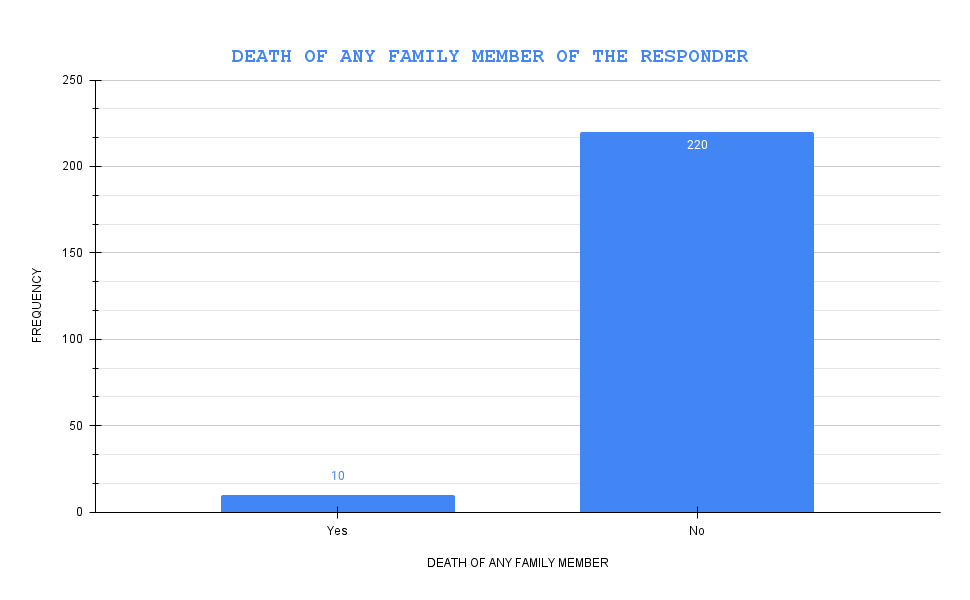
\includegraphics[width=0.45\linewidth]{IMAGES/Image 27.png}
% 	\caption{Deaths due to Covid in Family}
% 	\label{G27}
% \end{figure}

% \ 

% In Figure \ref{G27}, it is observed that among the 230 participants, 10 individuals have encountered the loss of a family member due to covid.


% \newpage


% \section{Income Difference between Pre-Pandemic and Post-Pandemic Situation}

% \begin{figure}[h!]
% 	\centering
% 	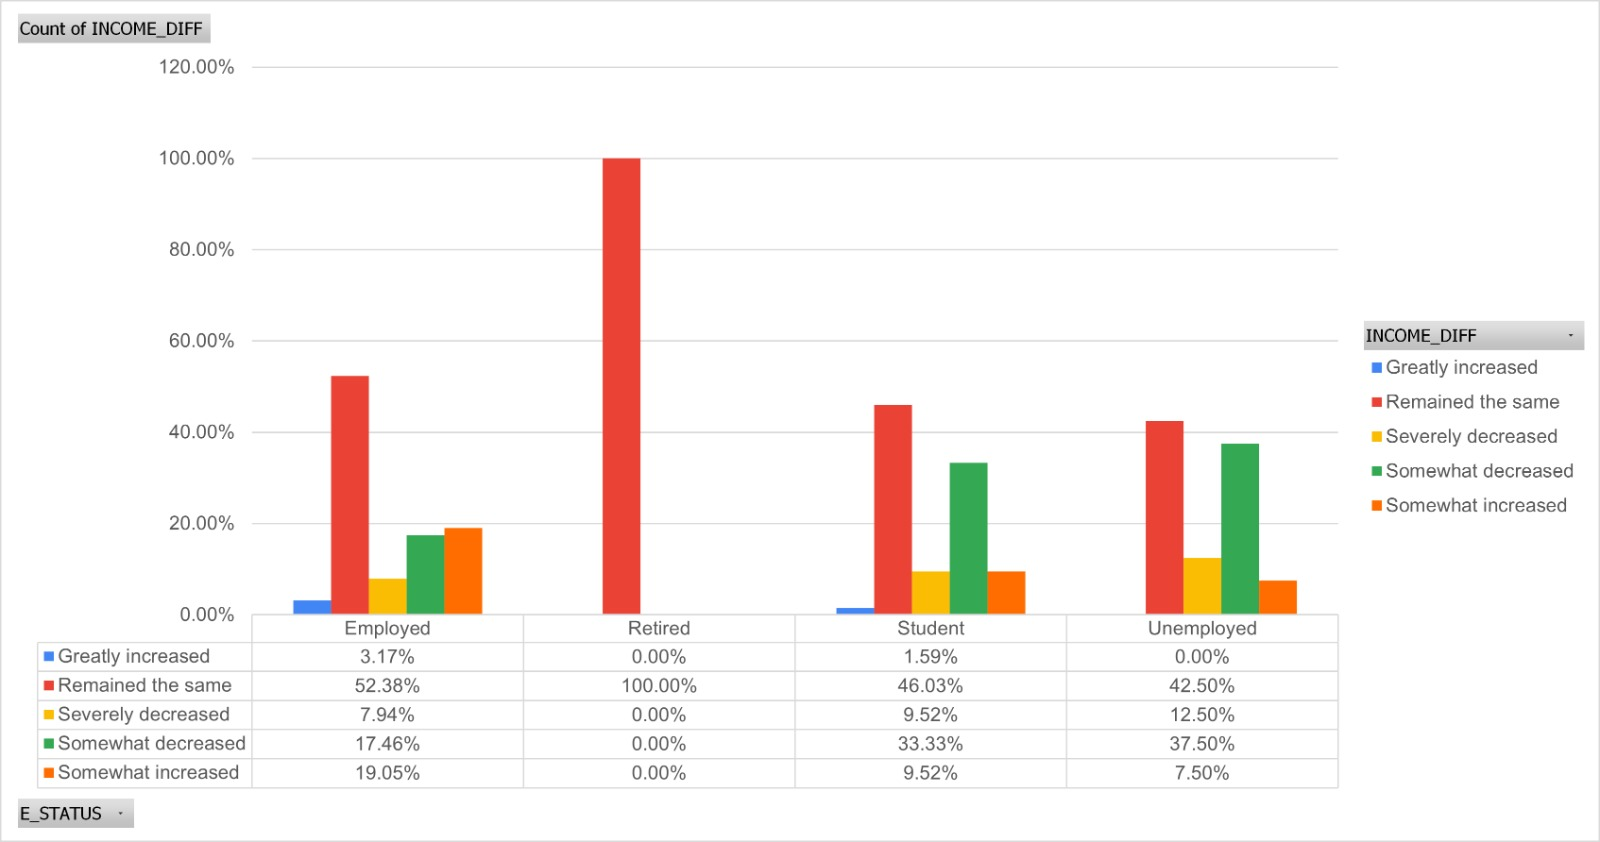
\includegraphics[width=0.8\linewidth]{IMAGES/Image 5.jpg}
% 	\caption{Difference in Incomes}
% 	\label{G5}
% \end{figure}
% $$\text{Employed(63) | Retired(1) | Student(126) | Unemployed(40)}$$

% \ 

% The bar graph in Figure \ref{G5} illustrates the difference in incomes between the pre-pandemic and post-pandemic period for participants with different employment status. It is measured in percentage. Overall it can be observed that the income remained almost same or somewhat decreased in each employment category.

% \ 

% Almost half of the participants with the employed, student and unemployed status had their salary unaffected and also the retired one. In the group of student and unemployed ones, $1/3^{rd}$  portion and among employed ones 17.46\%  had slight decrement in their income. Only a very small part in employed and student category claimed great increase in their income. About 10\% participant's salary got critically decreased. 


% \newpage

% \section{Comparison of Family Expenditure Across Different Employment Status}

% \begin{figure}[h!]
% 	\centering
% 	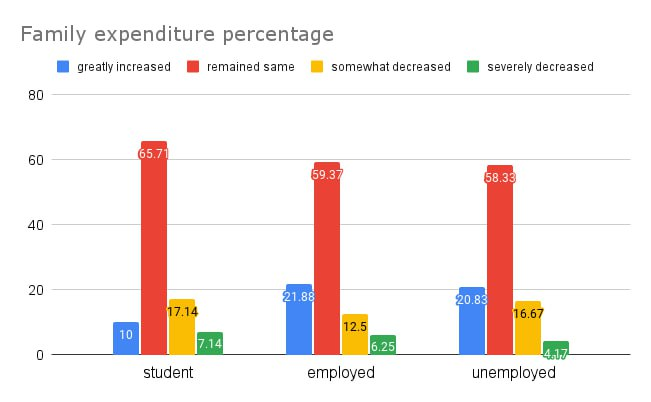
\includegraphics[width=0.9\linewidth]{IMAGES/Image 33.jpeg}
% 	\caption{Percentage of Family Expenditure}
% 	\label{G33}
% \end{figure}
% $$\text{Student(126) | Employed(63) | Unemployed(40)}$$

% \ 

% The bar chart depicts the distribution of family expenditure levels across three distinct categories of individuals: students, employed individuals, and the unemployed. Expenditure levels are classified into four groups: "Greatly Increased," "Remained Same," "Somewhat Decreased," and "Severely Decreased."\\
% Let’s analyze the Family Expenditure, So for students, 10\% experienced a substantial increase in family expenditure, while a majority (65.71\%) maintained a consistent level. Approximately 17.14\% observed a moderate decrease, and a smaller portion (7.14\%) faced a significant reduction.\\
% Among employed individuals, 21.88\% noted a substantial rise in family expenditure, while the largest portion (59.37\%) sustained a steady spending pattern. About 12.5\% experienced a moderate decline, and a smaller proportion (6.25\%) encountered a considerable drop.\\
% Unemployed individuals experienced noteworthy changes as well, with 20.83\% noting a significant increase, 58.33\% maintaining consistency, 16.67\% observing a moderate reduction, and a minority (4.17\%) facing a substantial decrease in family spending.

% \newpage 

% \textbf{Some key insights that can be drawn from the graph is that,}

% \ 

% Consistency Among Employees:  The largest percentage of both employed individuals and students maintained similar family expenditure levels, with around 59.37\% and 65.71\%, respectively, staying consistent.

% \ 

% Impact of Unemployment: Unemployed individuals showcased a slightly higher percentage in experiencing increased family expenditure (20.83\%) compared to employed individuals (21.88\%).

% \ 

% Variance in Decreased Expenditure: There is a notable difference in the percentage of individuals who experienced a severe decrease in family spending among the employed (6.25\%) compared to students (7.14\%) and the unemployed (4.17\%).

% \ 

% This breakdown of family expenditure across employment categories offers valuable insights into how different groups manage their expenses amidst varying employment statuses.

% \newpage

% \section{Comparative Analysis of Income Change Across Different Employment Categories}

% \begin{figure}[h!]
% 	\centering
% 	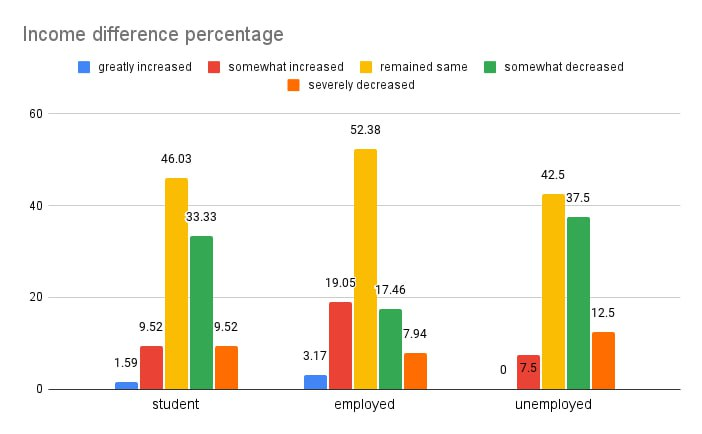
\includegraphics[width=0.9\linewidth]{IMAGES/Image 34.jpeg}
% 	\caption{Percentage of Differences in Incomes}
% 	\label{G34}
% \end{figure}
% $$\text{Student(126) | Employed(63) | Unemployed(40)}$$

% \ 

% The bar chart provides an overview of income change percentages across three distinct categories of individuals: students, employed individuals, and the unemployed. The income change percentages are divided into five groups: "Greatly Increased", "Somewhat Increased", "Remained Same", "Somewhat Decreased", and "Severely Decreased".

% \ 

% In the case of students, 1.59\% experienced a significant increase in income, while 9.52\% observed a moderate rise. A substantial majority of students (46.03\%) maintained a consistent income level, with approximately 33.33\% facing a moderate decrease and 9.52\% encountering a substantial reduction.

% \ 

% Among employed individuals, 3.17\% saw a notable increase in income, and 19.05\% experienced a moderate rise. The largest portion of employed individuals (52.38\%) sustained a steady income level, while around 17.46\% observed a moderate decline, and 7.94\% faced a substantial reduction.

% \ 

% For unemployed individuals, none experienced a significant increase, and 7.5\% observed a moderate rise. A significant majority (42.5\%) maintained a consistent income level, while around 37.5\% experienced a moderate decrease, and 12.5\% encountered a substantial reduction.

% \ 

% Analyzing these figures reveals that the largest percentage of employed individuals (52.38\%) maintained a steady income level, surpassing both students (46.03\%) and unemployed individuals (42.5\%). Moreover, a notable portion of students (33.33\%) faced a moderate decrease in income, exceeding the corresponding percentages for employed and unemployed individuals.

% \ 

% It is noteworthy that the percentage of unemployed individuals experiencing any level of increased income (7.5\%) is notably lower compared to students (11.11\%) and employed individuals (22.22\%). This breakdown of income change percentages across employment categories provides insights into the varying income dynamics experienced by different groups based on their employment status.


% \newpage

% \section{Income and Expenses During Covid}

% \begin{figure}[h!]
% 	\centering
% 	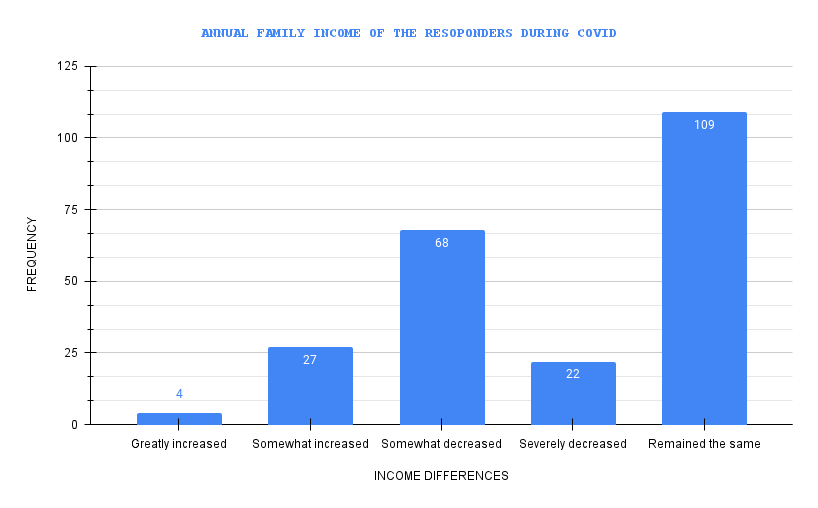
\includegraphics[width=0.65\linewidth]{IMAGES/Image 19.png}
% 	\caption{Income and Expenses}
% 	\label{G19}
% \end{figure}

% \ 

% \begin{figure}[h!]
% 	\centering
% 	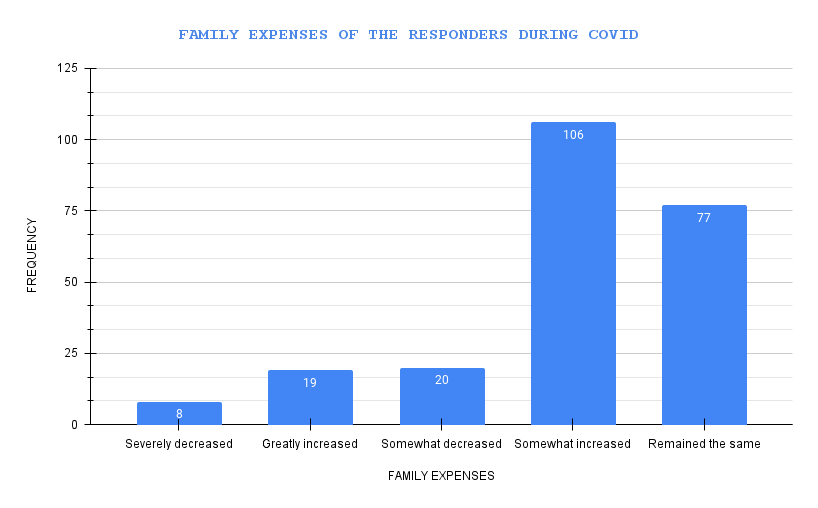
\includegraphics[width=0.65\linewidth]{IMAGES/Image 20.png}
% 	\caption{Income and Expenses}
% 	\label{G20}
% \end{figure}

% \ 

% Figure \ref{G19} indicates the fluctuations in annual family income among respondents during the COVID-19 pandemic. The majority, that is, 109 participants have reported no significant change in their family income. However, 68 participants experienced a slight decrease, while 22 participants faced a substantial decrease in income. On a positive note, 27 participants saw a moderate increase, and 4 participants reported a significant boost in their annual family income.

% \ 

% However, for the majority of participants, monthly family expenses have either remained constant or experienced a slight increase. Figure \ref{G20} shows that for 106 participants, the monthly expenses have somewhat increased, while for 77 participants, family expenditures have stayed the same.


% \newpage

% \section{Dependence on Cooked Food Delivery System during COVID}

% \begin{figure}[h!]
% 	\centering
% 	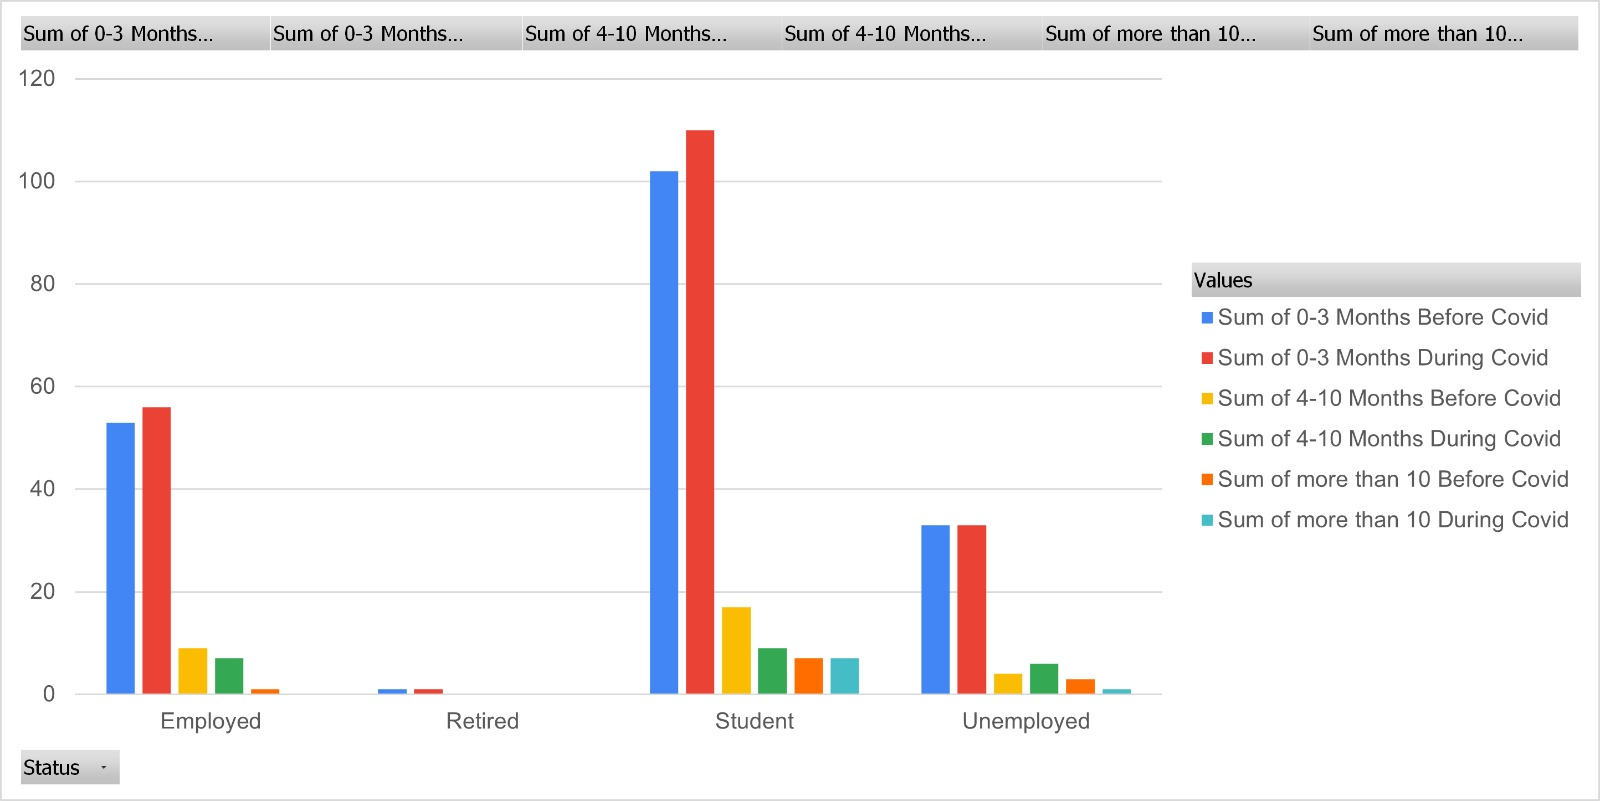
\includegraphics[width=0.9\linewidth]{IMAGES/Image 6.jpg}
% 	\caption{Dependence on Cooked Food Delivery System}
% 	\label{G6}
% \end{figure}
% $$\text{Employed(63) | Retired(1) | Student(126) | Unemployed(40)}$$

% \ 

% Figure \ref{G6} represents the change in ‘Dependence on cooked-food delivery system’ due to pandemic for participants corresponding to several employment status. It is measured in corresponding frequency. 

% \ 

% From the mere observation, it can be seen that there has been some upward trend in the \textbf{“0-3 times per month}” segment among the student and employed participants. Whereas the no. of unemployed and retired ones in this segment remained same as before COVID.\\ \\
% The no. of students and employed persons in the “\textbf{4-10 times per month}” segment gets slightly decreased while the no. Of unemployed ones in this segment got slightly increased.\\ \\ 
% In the “\textbf{More than 10 times per month}” the students did not show any change of habit, while employed and unemployed ones reduced their order frequency. It should also be noted that there has been lest no. Of participants in this segment during COVID as well as before COVID. 

% \newpage

% \begin{figure}[h!]
% 	\centering
% 	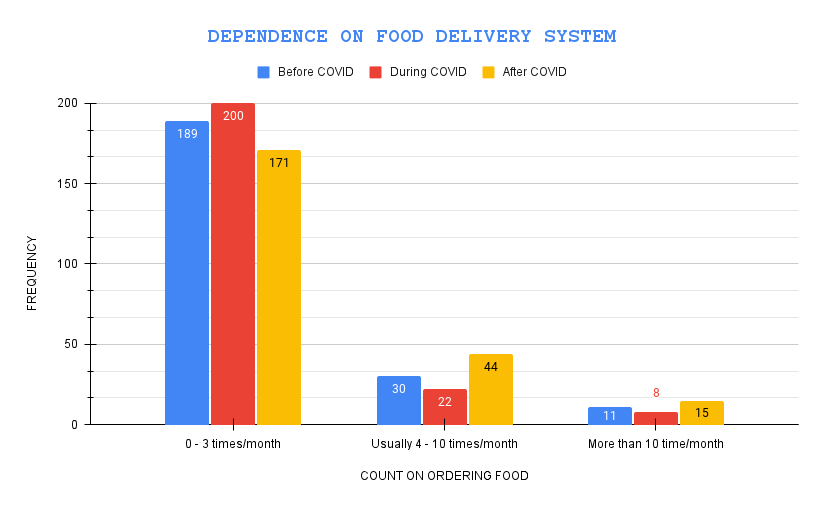
\includegraphics[width=0.9\linewidth]{IMAGES/Image 13.png}
% 	\caption{Dependence on Cooked Food Delivery System}
% 	\label{G13}
% \end{figure}

% \ 

% \begin{figure}[h!]
% 	\centering
% 	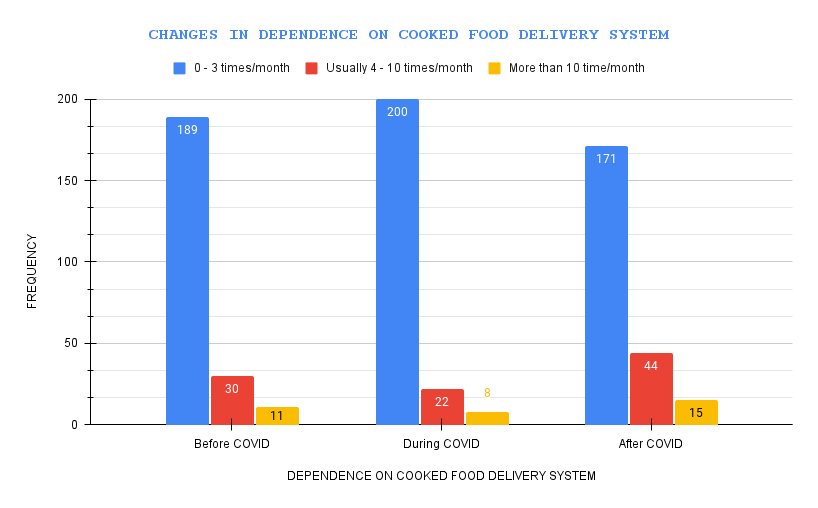
\includegraphics[width=0.9\linewidth]{IMAGES/Image 14.png}
% 	\caption{Dependence on Cooked Food Delivery System}
% 	\label{G14}
% \end{figure}

% \ 


% Figure \ref{G13} and figure \ref{G14} illustrate a comparison between the number of times the participants ordered food online in a month before, during and after COVID-19. The majority of participants, regardless of the pandemic, exhibit a trend of ordering food online 0-3 times per month.

% \newpage

% \begin{figure}[h!]
% 	\centering
% 	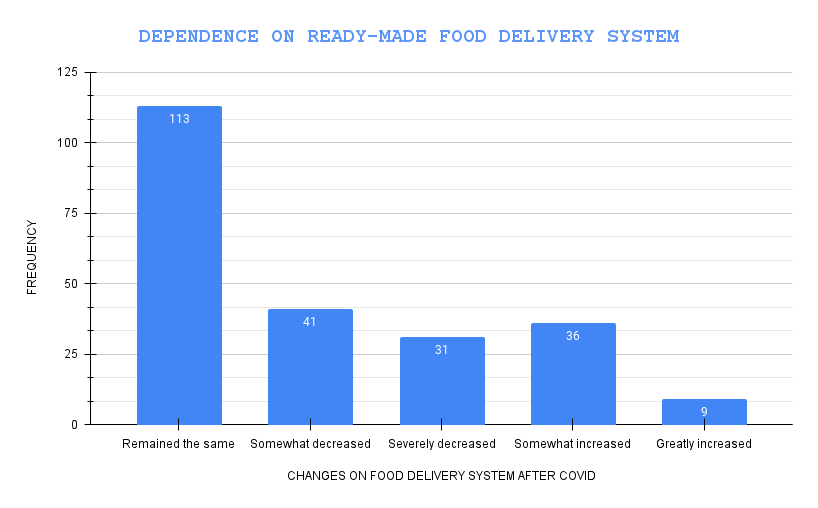
\includegraphics[width=0.9\linewidth]{IMAGES/Image 15.png}
% 	\caption{Dependence on Cooked Food Delivery System}
% 	\label{G15}
% \end{figure}

% \

% The data provided in Figure 4.3 illustrates the frequency dependence on ready-made food delivery systems. The majority of the respondents reported that their dependence on ready-made food delivery remained the same, while a smaller percentage indicated a somewhat decreased dependence and an even smaller percentage reported a severe decrease in dependence. Conversely, some respondents mentioned a somewhat increased dependence on ready-made food delivery, but the number of responses with greatly increased dependence has been very low.

% \ 

% This data mostly indicates two aspects of thought processes adapted by people during the COVID-19 Lockdown period. A significant number of families believed that the Virus could be carried through right into the house with the ready-made food despite all the precaution and contactless delivery etc. Hence, the chances of contamination may increase. Therefore, they somewhat decreased ordering ready-made food. On the other hand, a significant amount of people felt the need of ordering ready-made food more often than before. This may be due to lack of availability of raw cooking materials during the Lockdown period, or it might be safe to say that a few got addicted to an easier lifestyle that the pandemic offered.

% \newpage

% \section{Vaccination Status}

% \begin{figure}[h!]
% 	\centering
% 	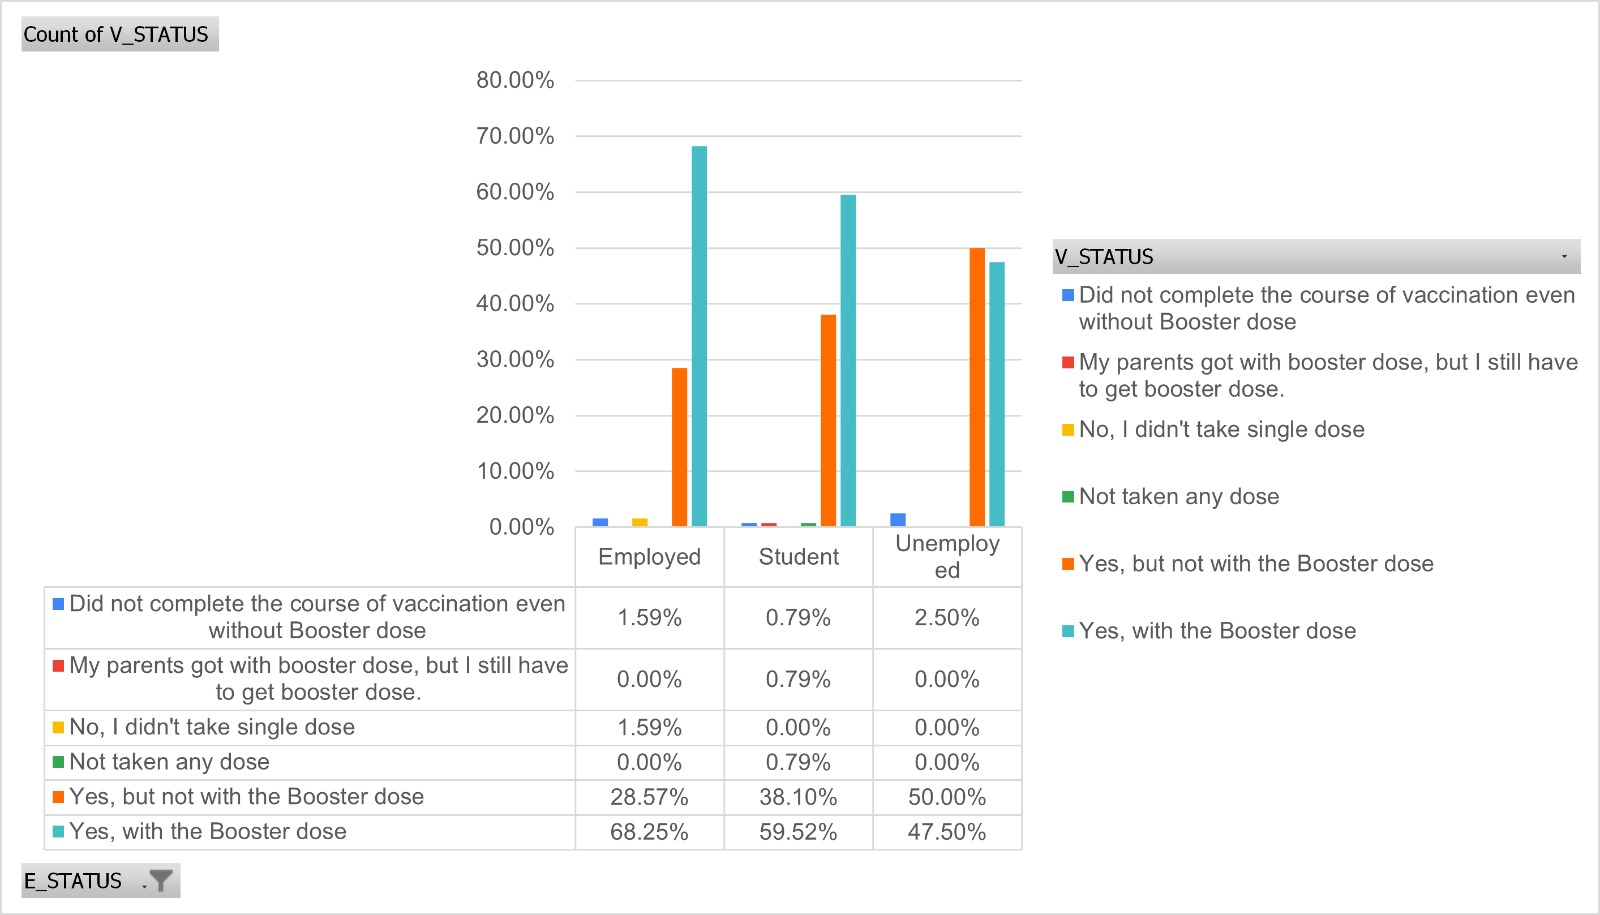
\includegraphics[width=0.9\linewidth]{IMAGES/Image 7.jpg}
% 	\caption{Vaccination Status}
% 	\label{G7}
% \end{figure}
% $$\text{Employed(63) | Student(126) | Unemployed(40)}$$
% \ 
% \\
% The bar graph in Figure \ref{G7} illustrates the vaccination status for participants with different employment condition. It has been measured in percentage.

% \ 

% There is 1.59\% employed participants who did not take any dose and a same portion with incomplete course of vaccination.  The majority of employed participants (68.25\%) finished the vaccination with booster dose and 28.57\% without booster dose.\\ \\ 
% It can be observed that a very small portion of students either did not take the booster dose or  any dose. About 59.52\% of students got properly vaccinated and the remaining 38.10\% are to be vaccinated with the booster dose.\\ \\ 
% Among the unemployed participants only 2.50\% did not complete the vaccination process. While half of them got vaccinated without booster dose, 47.5\% completed the vaccination with booster dose.\\ \\ 
% It can be seen that almost all the participants are either fully vaccinated with booster dose or without booster dose.

% \

% \newpage

% \section{Medical Expenses during COVID}

% \begin{figure}[h!]
% 	\centering
% 	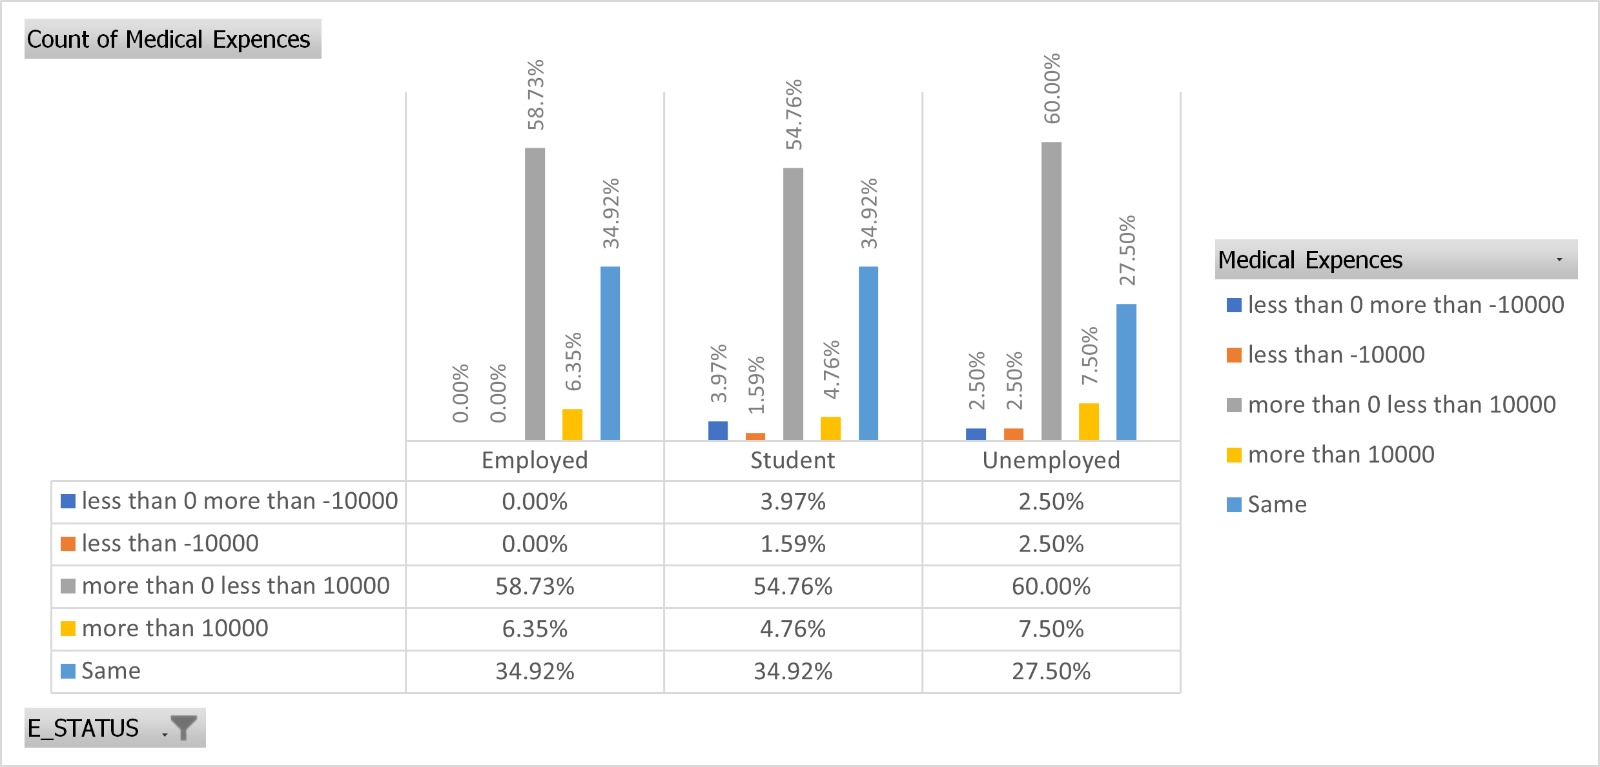
\includegraphics[width=0.85\linewidth]{IMAGES/Image 8.jpg}
% 	\caption{Count of Medical Expenses}
% 	\label{G8}
% \end{figure}
% $$\text{Employed(63) | Student(126) | Unemployed(40)}$$

% \ 

% Figure \ref{G8} shows that among employed candidates medical expenses of their family after pandemic decrease more than ten thousand 0\% of employed candidates , medical expenses of their family after pandemic decrease between zero and ten thousand 0\% of employed candidates , medical expenses of their family after pandemic increase more than ten thousand 6.35\% of employed candidate , medical expenses of their family increase after pandemic between zero and ten thousand 58.73\% of employed candidates and medical expenses of their family after pandemic remained unchanged for 34.92\% of employed candidates.
% \\ \\
% Among students medical expenses of their family after pandemic decrease more than ten thousand 1.59\% of students , medical expenses of their family after pandemic decrease between zero and ten thousand 3.97\% of students , medical expenses of their family after pandemic increase more than ten thousand 4.76\% of students, medical expenses of their family after pandemic increase between zero and ten thousand 54.76\% of students and medical expenses of their family after pandemic remained unchanged for 34.92\% of students.\\ \\
% Among unemployed candidates medical expenses of their family after pandemic decrease more than ten thousand 2.50\% of unemployed candidates, medical expenses of their family after pandemic decrease between zero and ten thousand 2.50\% of unemployed candidates, medical expenses of their family after pandemic increase more than ten thousand 7.50\% of unemployed candidate, medical expenses of their family after pandemic increase between zero and ten thousand 60\% of unemployed candidates and medical expenses of their family after pandemic remained unchanged for 27.50\% of unemployed candidates.

% \newpage 

% \section{Weight Difference between Pre and Post-Pandemic Situations}

% \begin{figure}[h!]
% 	\centering
% 	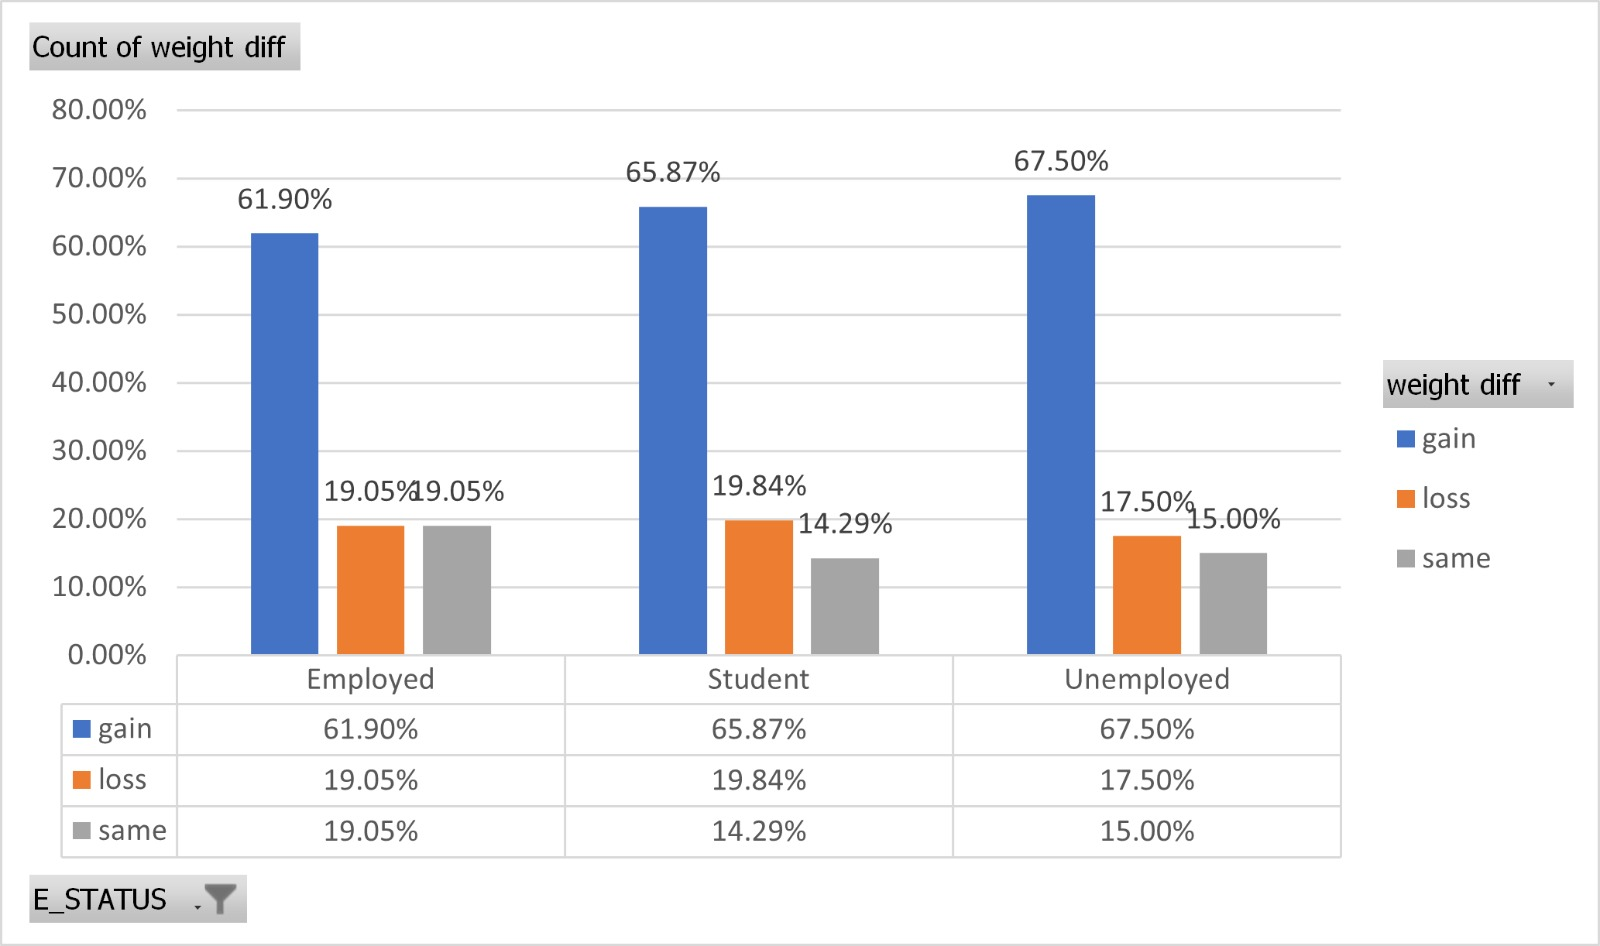
\includegraphics[width=0.9\linewidth]{IMAGES/Image 9.jpg}
% 	\caption{Count of Weight Difference}
% 	\label{G9}
% \end{figure}
% $$\text{Employed(63) | Student(126) | Unemployed(40)}$$

% \ 

% Figure \ref{G9} shows that among employed candidates 61.90\% of employed candidates gained weight during pandemic \\ (COVID-19) and 19.05\% of employed candidate lost weight during pandemic and the weight remained same for 19.05\% of employed candidates during pandemic.

% \ 

% Among students 65.87\% of students gained weight during pandemic (COVID -19) and 19.84\% of students lost weight during pandemic and the weight remained same for 14.29\% of students during pandemic.\\
% Among unemployed candidates 67.50\% of unemployed candidates gained weight during pandemic (COVID-19) and 17.50\% of unemployed candidate lost weight during pandemic and the weight remained same for 15.00\% of unemployed candidates during pandemic.


% \newpage

% \section{Going Outside and Social Interaction}

% \begin{figure}[h!]
% 	\centering
% 	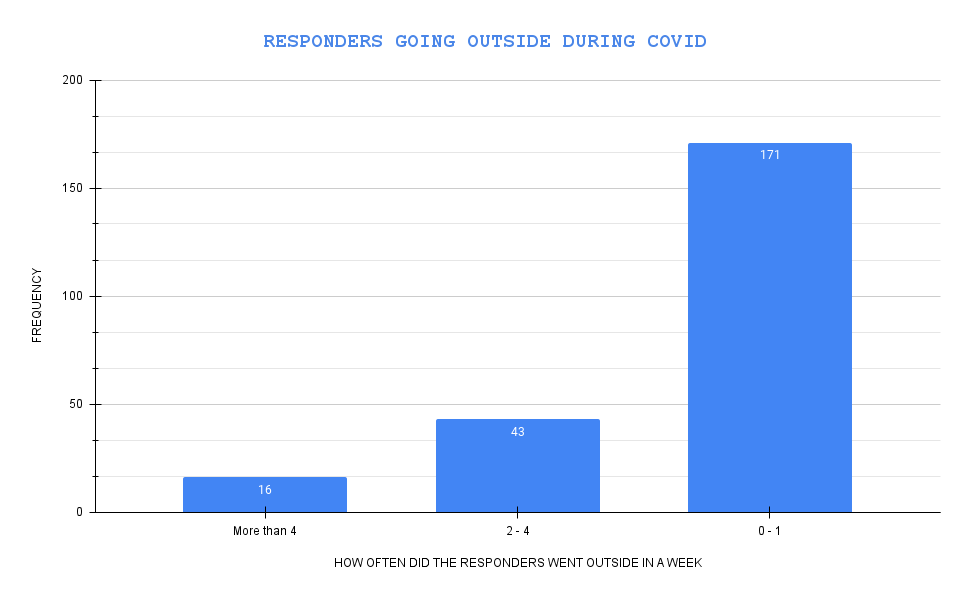
\includegraphics[width=0.68\linewidth]{IMAGES/Image 22.png}
% 	\caption{Going Outside}
% 	\label{G22}
% \end{figure}

% \ 

% Due to the impact of COVID-19, the frequency of going out has undergone a substantial change. From figure \ref{G22} we see that among the 230 participants surveyed, 171 individuals reported going out at most once a week during the pandemic.

% \ 

% \begin{figure}[h!]
% 	\centering
% 	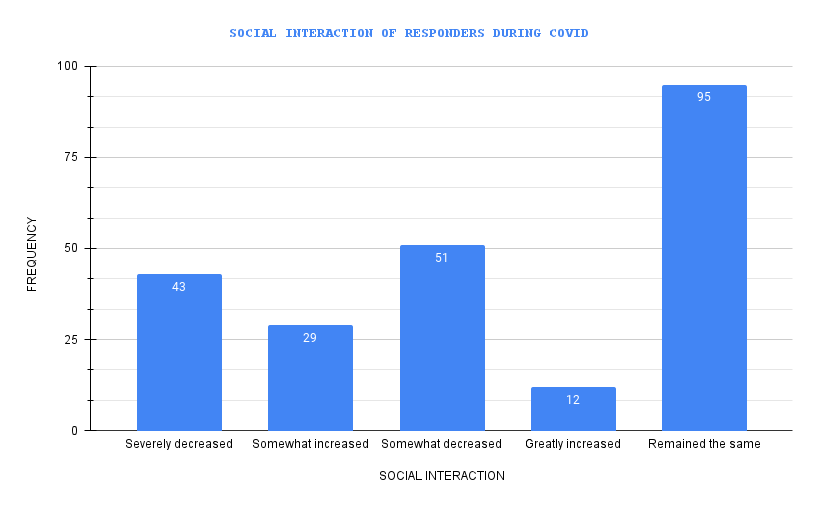
\includegraphics[width=0.68\linewidth]{IMAGES/Image 23.png}
% 	\caption{Social Interaction}
% 	\label{G23}
% \end{figure}

% Clearly it has also affected social interaction. Figure \ref{G23} illustrates that the social interaction of 43 people has markedly diminished, while 29 people have experienced a modest increase. For 51 individuals, social engagement has somewhat decreased, whereas 12 people have seen a notable rise in their social interactions. Remarkably, the social interactions of 95 people have remained unchanged.


% \newpage

% \section{Screen-time Percentage during COVID}

% \begin{figure}[h!]
% 	\centering
% 	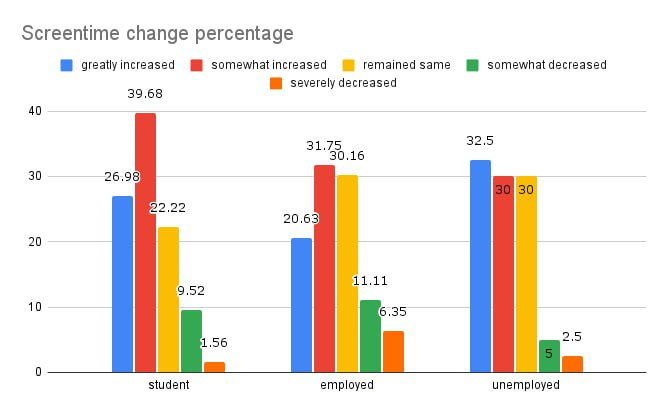
\includegraphics[width=0.9\linewidth]{IMAGES/Image 10.jpeg}
% 	\caption{Screen-time Percentage}
% 	\label{G10}
% \end{figure}
% $$\text{Student(126) |Employed(63) | Unemployed(40)}$$

% \ 

% Figure \ref{G10} represents the screen time changes for different categories of people during COVID-19. It indicates that across all categories, screen time has somewhat increased to a large extent.

% \ 

% For students, employees and unemployed, the percentages are 39.68\%, 31.75\% and 30\%, respectively. Additionally, a significant percentage increase is observed for people from different categories, with percentages of 26.98\%, 20.63\% and 32.5\% for students, employees and unemployed respectively.\\ \\
% The data also reveals that screen time has remained the same for a substantial number of people. An interesting observation is that among those experiencing a significant increase in screen time, the proportion is highest for unemployed individuals, followed by students and employed individuals in decreasing order.

% \newpage

% \begin{figure}[h!]
% 	\centering
% 	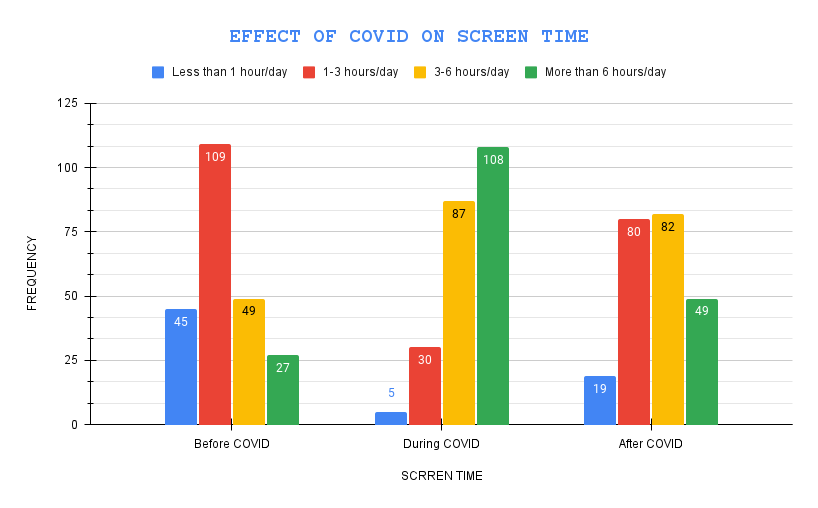
\includegraphics[width=0.9\linewidth]{IMAGES/Image 16.png}
% 	\caption{Screen-time Percentage}
% 	\label{G16}
% \end{figure}

% \ 

% The information presented in Figure \ref{G16} illustrates a comparison of daily screen time during distinct time periods—before, during and after the COVID-19 pandemic.

% \ 

% \begin{figure}[h!]
% 	\centering
% 	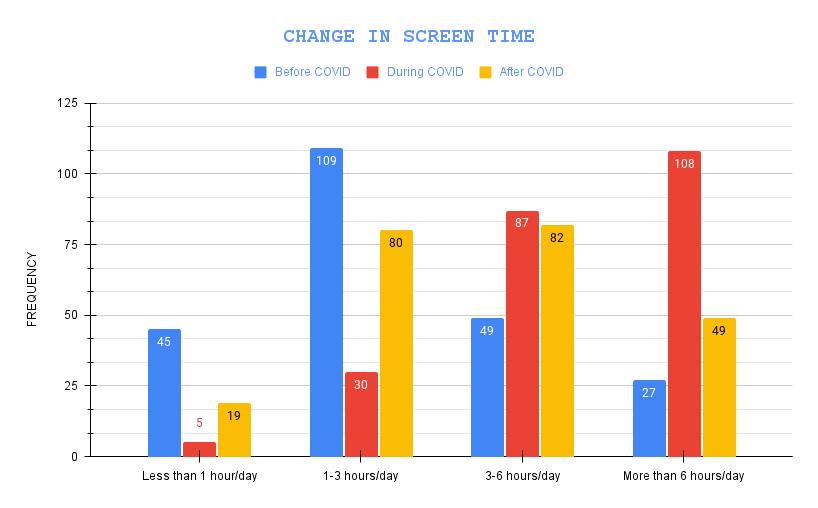
\includegraphics[width=0.9\linewidth]{IMAGES/Image 17.png}
% 	\caption{Screen-time Percentage}
% 	\label{G17}
% \end{figure}

% \newpage

% Figure \ref{G17} presents a visual representation comparing the number of people having a particular limit of screen time before, during and after the COVID-19.

% \ 

% Before COVID-19, the majority of participants reported engaging in screen time for 1-3 hours per day. However, with the advent of the pandemic, there has been a notable and significant increase in the number of individuals spending more than 6 hours per day on screens. Also, the proportion of people with less than 1 hour of screen time per day during this period has diminished considerably. Post-COVID-19, a substantial portion of participants now falls within the range of 1-6 hours of daily screen time.

% \ 

% \begin{figure}[h!]
% 	\centering
% 	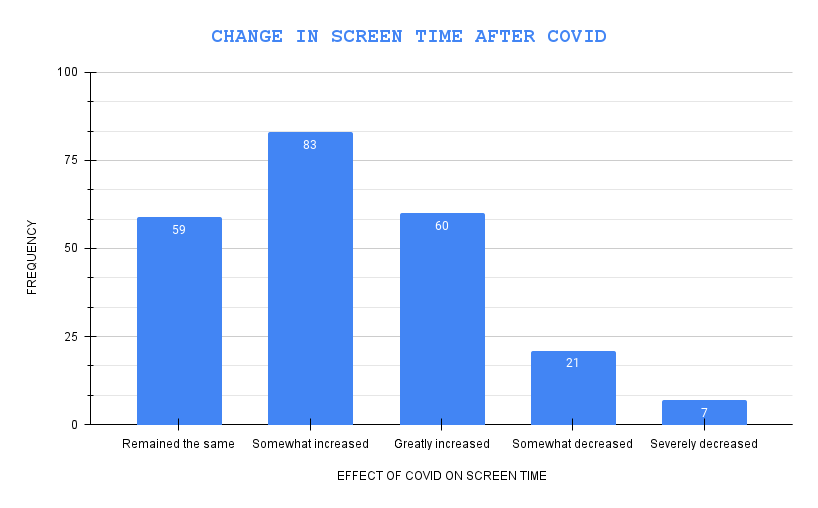
\includegraphics[width=0.9\linewidth]{IMAGES/Image 18.png}
% 	\caption{Screen-time Percentage}
% 	\label{G18}
% \end{figure}

% \ 

% Figure \ref{G18} shows that for majority of the participants the screen time has somewhat increased during covid 19. 


% \newpage

% \section{Mental Health Percentage during COVID}

% \begin{figure}[h!]
% 	\centering
% 	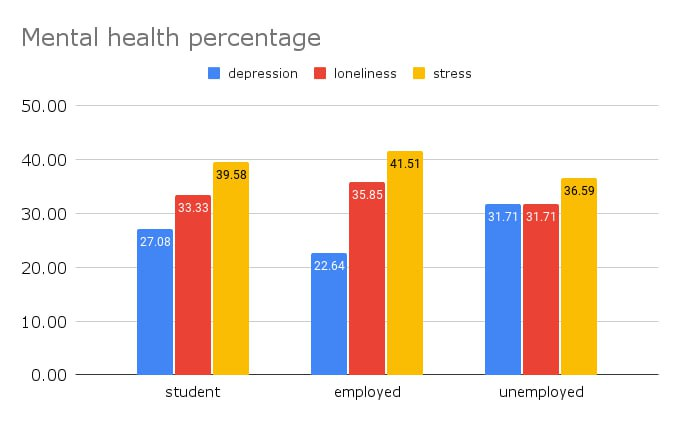
\includegraphics[width=0.9\linewidth]{IMAGES/Image 11.jpeg}
% 	\caption{Mental Health Percentage}
% 	\label{G11}
% \end{figure}
% $$\text{Student(126) |Employed(63) | Unemployed(40)}$$

% \ 

% Figure \ref{G11} represents the mental health status of different categories during COVID-19.

% \ 

% It shows that 39.5\% of students, 41.51\% of employed individuals, and 36.59\% of unemployed persons were experiencing stress. A significant number of people were also dealing with loneliness, with rates of 33.33\% for students, 35.85\% for employed individuals, and 31.71\% for the unemployed. Additionally, 27.08\% of students, 22.64\% of employed individuals, and 31.71\% of unemployed persons have faced depression.\\ \\
% The above observations depict that almost everyone in all categories has gone through a mental health crisis. A sense of uncertainty and helplessness are the main reasons behind it. Loss of families, friends, jobs, and many more have pushed us towards another significant crisis—mental health.

% \newpage

% \begin{figure}[h!]
% 	\centering
% 	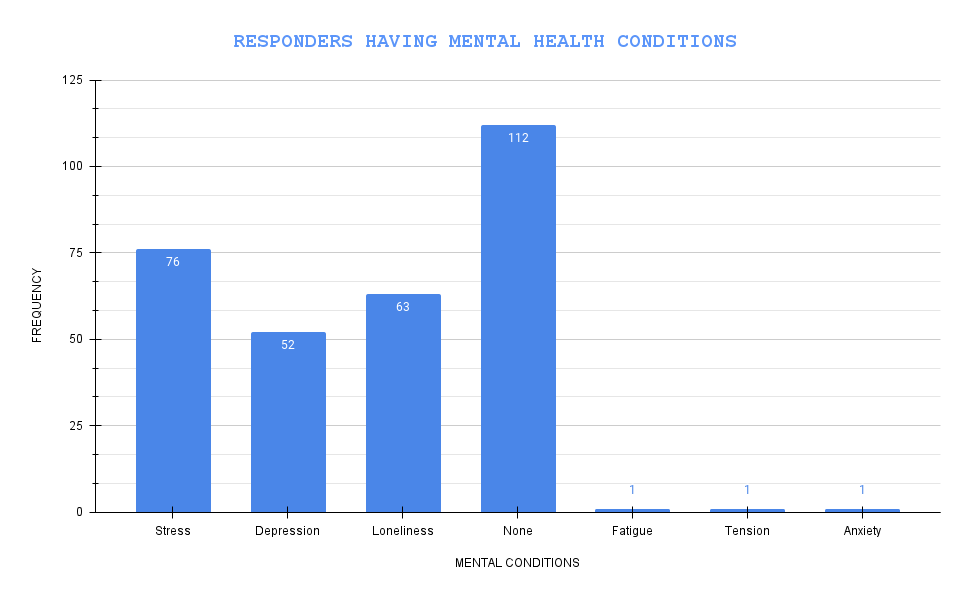
\includegraphics[width=0.9\linewidth]{IMAGES/Image 12.png}
% 	\caption{Mental Health Percentage}
% 	\label{G12}
% \end{figure}

% \

% Figure \ref{G12} shows the number of responders having mental health conditions during covid-19 pandemic. The predominant conditions reported were stress, loneliness and depression, affecting 76, 63 and 52 individuals, respectively. Noteworthy outliers included cases of fatigue, tension and anxiety. It is important to highlight that a substantial proportion of participants did not experience any mental health issues during this challenging time.


% \newpage

% \section{Effects on Education System}

% \begin{figure}[h!]
% 	\centering
% 	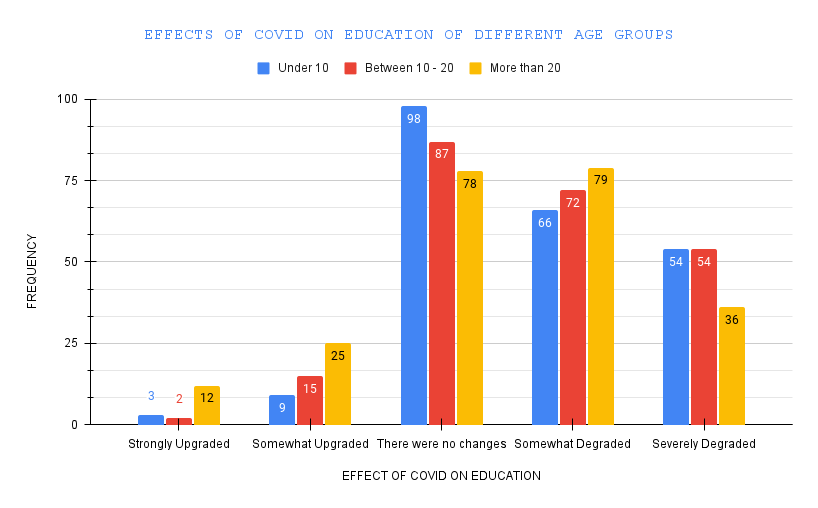
\includegraphics[width=0.9\linewidth]{IMAGES/Image 21.png}
% 	\caption{Effects on Education}
% 	\label{G21}
% \end{figure}

% \ 

% Figure \ref{G21} provides insights into the impact of Covid-19 on the education of various age groups. 

% \ 

% In conclusion, the data indicate that education among children under the age of 10 has either stayed consistent or has decreased in comparison to the pre-pandemic period. The quality of education has remained the same or has declined for children aged 10 to 20 and adult education has stayed stable or has deteriorated a bit.


% \newpage

% \section{Institutional Activities}

% \begin{figure}[h!]
% 	\centering
% 	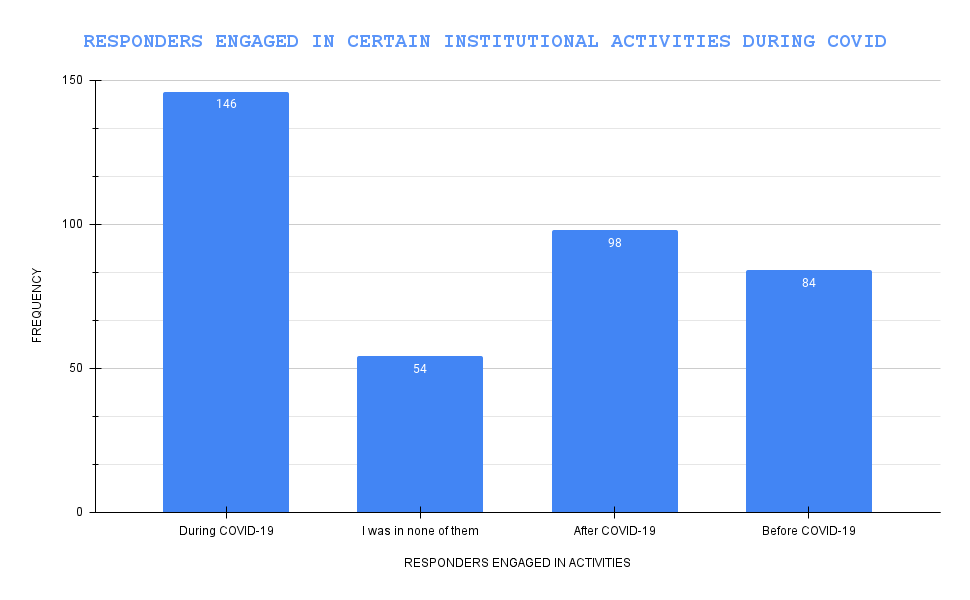
\includegraphics[width=0.65\linewidth]{IMAGES/Image 24.png}
% 	\caption{Institutional Activities}
% 	\label{G24}
% \end{figure}

% \ 

% Figure \ref{G24} displays the impact of the COVID-19 epidemic on responder participation in institutional activities. Before the pandemic, the frequency of engagement stood at 84, but during the pandemic, it soared to 146. Subsequently, post-pandemic, the frequency dropped to 98. This dynamic pattern demonstrates a significant increase in overall responder engagement during the pandemic. On the other hand, 54 respondents, remained uninvolved in any institutional activity for the entire period.

% \

% \section{Work from Home}

% \begin{figure}[h!]
% 	\centering
% 	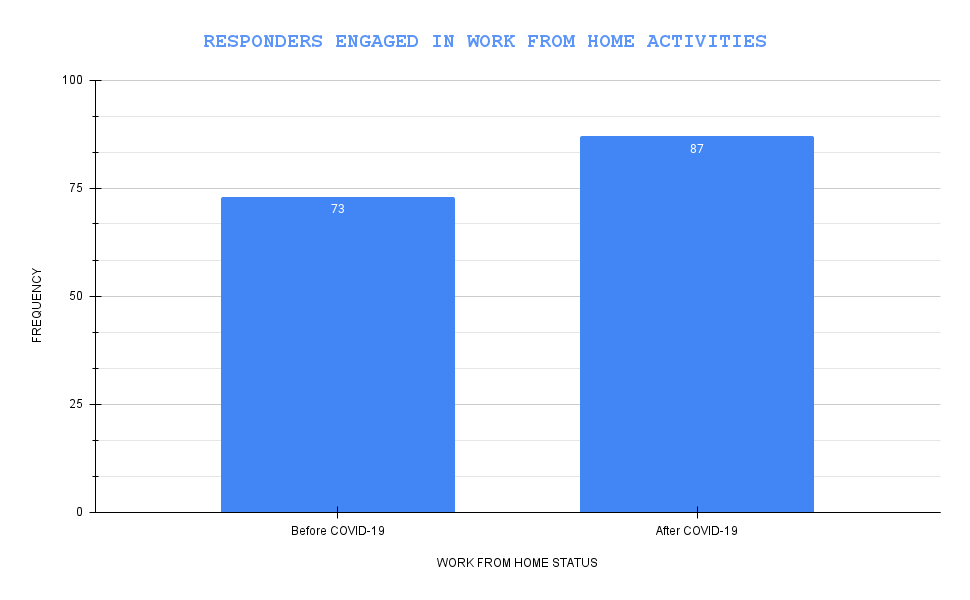
\includegraphics[width=0.5\linewidth]{IMAGES/Image 25.png}
% 	\caption{Work from Home}
% 	\label{G25}
% \end{figure}

% \ 

% Figure \ref{G25} Among participant 73 people used to work from home before covid-19 and after covid-19 the number of people work from home has increased to 87.


% \newpage

% \section{Analysis of Healthy Habits taken up by Individuals}

% \begin{figure}[h!]
% 	\centering
% 	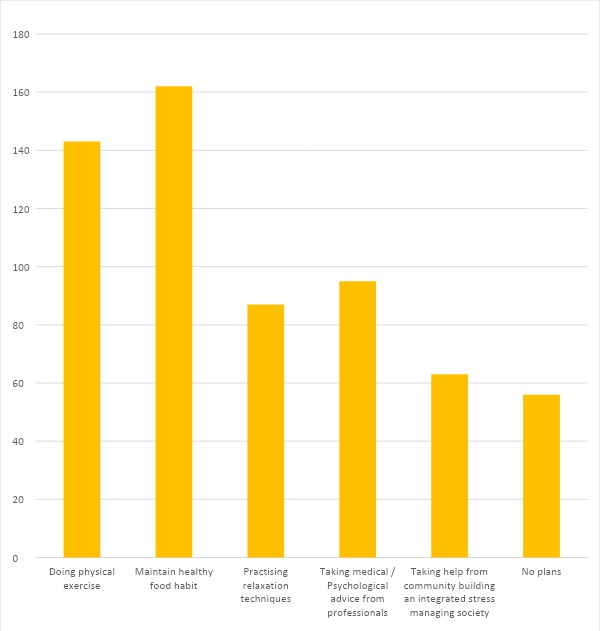
\includegraphics[width=0.9\linewidth]{IMAGES/Image 28.jpeg}
% 	\caption{Healthy Habits}
% 	\label{G28}
% \end{figure}

% \ 

% Analysis of the healthy habits taken up by the individuals reveals interesting trends among the 230 participants. A significant 70.43\% express a desire to maintain a healthy food habit, emphasizing the importance placed on nutrition in their overall well-being. Additionally, 62.17\% are keen on incorporating regular physical exercises into their routines, highlighting a conscious effort to stay physically active for optimal health.\\ \\

% Furthermore, the data indicates that 37.82\% of participants are inclined towards practicing relaxation techniques, showcasing a recognition of the importance of mental well-being. Notably, 41.30\% express a preference for seeking medical or psychological advice from professionals, indicating a proactive approach to managing their health through expert guidance.\\ \\  

% In an intriguing dimension, 27.39\% of individuals express a desire to seek support from their community in building an integrated stress management society to address the challenges posed by diseases. This reflects a community-oriented mindset in combating health issues collaboratively.\\ \\

% However, 24.34\% of the participants seem to lack pre-planning in adopting specific healthy habits. This highlights a potential area for intervention and education to raise awareness about the benefits of proactive health measures.
% \\ \\

% Insights drawn from the data underscore the prominence of individuals aiming to maintain both a healthy food habit and regular physical exercises, with percentages of 70.43\% and 62.17\%, respectively. This dual focus on nutrition and physical activity suggests a holistic approach to health, particularly in the context of combating severe pandemics.\\ \\

% As we navigate the challenges of the current pandemic, it becomes evident that having hygiene plans in place is a proactive measure against potential future epidemics, such as the possibility of another COVID-19-like situation within the next 20 years. The importance of developing personal and community hygiene strategies cannot be overstated, as these measures play a crucial role in mitigating the spread of infectious diseases and fostering a healthier society overall.\\ \\


% \newpage

% \section{Precautional Measures taken up by Individuals}

% \begin{figure}[h!]
% 	\centering
% 	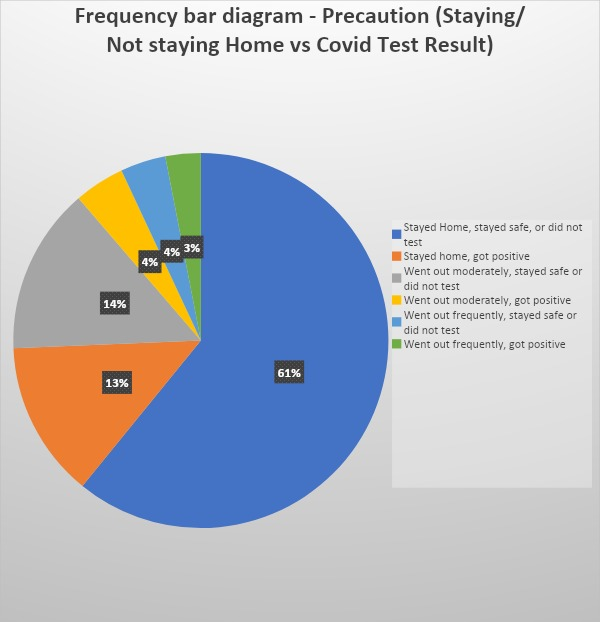
\includegraphics[width=0.7\linewidth]{IMAGES/Image 29.jpeg}
% 	\caption{Precautions taken}
% 	\label{G29}
% \end{figure}

% \ 

% \begin{figure}[h!]
% 	\centering
% 	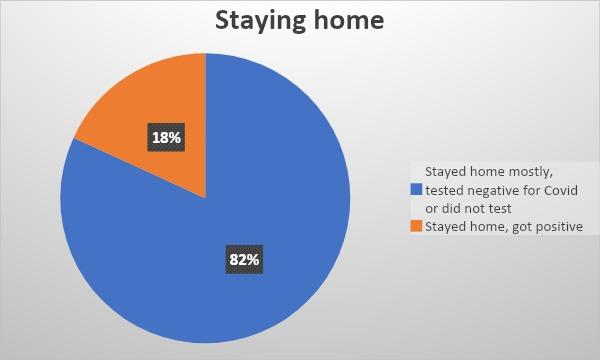
\includegraphics[width=0.7\linewidth]{IMAGES/Image 30.jpeg}
% 	\caption{Precautions taken}
% 	\label{G30}
% \end{figure}

% \ 

% \begin{figure}[h!]
% 	\centering
% 	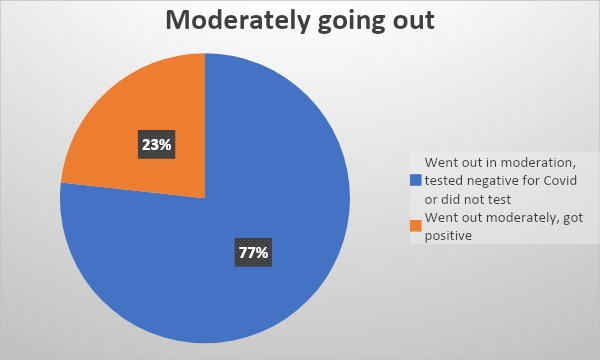
\includegraphics[width=0.7\linewidth]{IMAGES/Image 31.jpeg}
% 	\caption{Precautions taken}
% 	\label{G31}
% \end{figure}

% \ 

% \begin{figure}[h!]
% 	\centering
% 	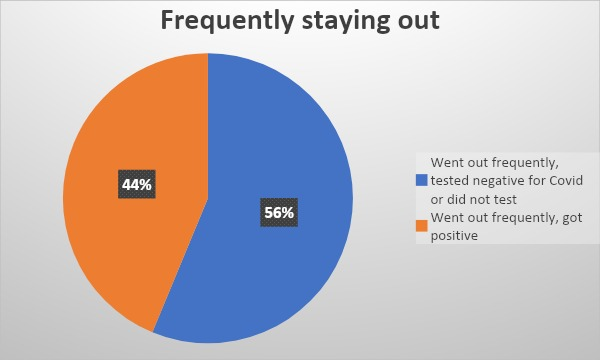
\includegraphics[width=0.7\linewidth]{IMAGES/Image 32.jpeg}
% 	\caption{Precautions taken}
% 	\label{G32}
% \end{figure}

% \ 

% The pie charts above provides an overview of the percentage distribution of a sample population across different categories related to staying at home during the COVID-19 pandemic. Approximately 61\% of individuals mostly stayed at home and remained untouched by COVID infection. Another 14\% of individuals contracted COVID while staying at home for reasons unknown. Additionally, about 14\% of the population ventured out moderately during the COVID pandemic and either stayed negative or did not get tested. A small percentage (4\%) of individuals who went out moderately got infected by the COVID virus. The percentage of people who frequently went out was small, and 4\% of them either stayed safe or did not get tested. Only 3\% of the population that went out frequently got infected with COVID.

% \ 

% Analyzing the pie chart, it becomes evident that staying at home played a crucial role in preventing the spread of COVID-19. Only 18\% of the sample population staying at home were infected, while 82\% remained mostly safe. The next pie chart illustrates the infection spread due to moderate outings, showing that 23\% of the sample population got infected due to moderate outings during the COVID pandemic. In the last pie chart, the results of frequently staying out are shown to contribute significantly to the increase in the spread of COVID infection, rising to 44\%. This suggests that going out frequently led to a higher risk of contamination.

% \ 

% The insights derived from the data are noteworthy. Staying at home emerged as a significant factor in preventing the spread of COVID and getting infected, as evidenced by the relatively low infection rate of 18\%. However, as people went out moderately from home, the rate of infection and positive cases increased by 5\%, indicating a relatively lower impact of moderate outings. Overall, the survey depicts that frequently staying out is a major factor contributing to the spread of COVID. Due to this factor, the infection rate rose by 26\% compared to staying at home.